 \let\negmedspace\undefined
\let\negthickspace\undefined
\documentclass[journal]{IEEEtran}
\usepackage[a5paper, margin=10mm, onecolumn]{geometry}
%\usepackage{lmodern} % Ensure lmodern is loaded for pdflatex
\usepackage{tfrupee} % Include tfrupee package

\setlength{\headheight}{1cm} % Set the height of the header box
\setlength{\headsep}{0mm}     % Set the distance between the header box and the top of the text
\usepackage{gvv-book}
\usepackage{gvv}
\usepackage{cite}
\usepackage{amsmath,amssymb,amsfonts,amsthm}
\usepackage{algorithmic}
\usepackage{graphicx}
\usepackage{textcomp}
\usepackage{xcolor}
\usepackage{txfonts}
\usepackage{listings}
\usepackage{enumitem}
\usepackage{mathtools}
\usepackage{gensymb}
\usepackage{comment}
\usepackage[breaklinks=true]{hyperref}
\usepackage{tkz-euclide} 
\usepackage{listings}
% \usepackage{gvv}                                        
\def\inputGnumericTable{}                                 
\usepackage[latin1]{inputenc}                                
\usepackage{color}                                            
\usepackage{array}                                            
\usepackage{longtable}                                       
\usepackage{calc}                                             
\usepackage{multirow}                                         
\usepackage{hhline}                                           
\usepackage{ifthen}                                           
\usepackage{lscape}



\usepackage{amsmath,amssymb}
\usepackage{booktabs}
\usepackage{tikz}
\usetikzlibrary{arrows.meta,angles,quotes}





\begin{document}

\bibliographystyle{IEEEtran}
\vspace{3cm}

\title{7.2.18}
\author{AI25BTECH11023 - Pratik R}
% \maketitle
% \newpage
% \bigskip
{\let\newpage\relax\maketitle}

\renewcommand{\thefigure}{\theenumi}
\renewcommand{\thetable}{\theenumi}
\setlength{\intextsep}{10pt} % Space between text and floats


\numberwithin{equation}{enumi}
\numberwithin{figure}{enumi}
\renewcommand{\thetable}{\theenumi}


\section*{\textbf{Question}}
Find the equation of the circle passing through $(0, 0)$ and making intercepts $a$ and $b$ on the coordinate axes.


\subsection*{\textbf{Solution}}

Let:
\begin{align}
\vec{x_1} = \myvec{0 \\ 0},\ \vec{x_2} = \myvec{a \\ 0},\ \vec{x_3} = \myvec{0 \\ b}
\end{align}

We use the general matrix form of a circle:


\begin{align}
\myvec{2x_1 & 2x_2 & 2x_3\\
1 & 1 & 1}^T \myvec{\vec{u} \\ f} = - \myvec{\norm{x_1}^2 \\ \norm{x_2}^2 \\ \norm{x_3}^2}
\end{align}

Substituting the values:

\begin{align}
\myvec{
0 & 0 & 1 \\
2a & 0 & 1 \\
0 & 2b & 1
}
\myvec{
u_1 \\
u_2 \\
f
}
=
- \myvec{
0 \\
a^2 \\
b^2
}
\end{align}

Using augmented matrix and

applying $R_1\leftrightarrow R_2$

and $R_2\leftrightarrow R_3$

\begin{align}
\myvec{
2a & 0 & 1 &\vrule &-a^2 \\ 
0 & 2b & 1 &\vrule &-b^2\\
0 & 0 & 1 &\vrule &0 
} \xleftrightarrow{R_1=R_1 - R_3}\xleftrightarrow{R_2=R_2 - R_3}
\myvec{
2a & 0 & 0 &\vrule &-a^2 \\ 
0 & 2b & 0 &\vrule &-b^2\\
0 & 0 & 1 &\vrule &0 
}
\end{align}

Solving the system:

\begin{align*}
f &= 0 \\
2a u_1 &= -a^2 \Rightarrow u_1 = -\frac{a}{2} \\
2b u_2 &= -b^2 \Rightarrow u_2 = -\frac{b}{2}
\end{align*}
\newpage
we get

\begin{align}
\vec{u} = \myvec{ -\frac{a}{2} \\ -\frac{b}{2} }, \quad f = 0
\end{align}

So the equation of the circle becomes:

\begin{align}
x^2 + y^2 + ax + by = 0
\end{align}

\begin{figure}[H]
\centering
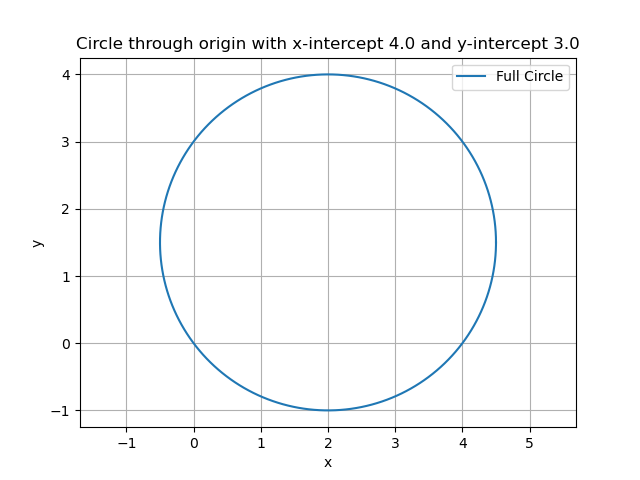
\includegraphics[width=0.7\columnwidth]{figs/fig.png} 
\caption{plane}
\label{}
\end{figure}

\end{document}
